\chapter{Navier-Stokes equation -- 2D -- Driven Cavity}

\modinfo{Directory}{DrivenCavity}
\modinfo{Solvers}{\Idx{FlowSolve}}
\modinfo{Tools}{\Idx{ElmerGrid}, \Idx{ElmerGUI}}
\modinfo{Dimensions}{2D, Steady-state}
\modinfo{Author}{Evangelos Voyiatzis}


\subsection*{Introduction}

This simple tutorial illustrates the application of Elmer to computational fluid dynamics problems.
The computational mesh is generated using the ElmerGrid utility while the model definition and its solution are carried out via ElmerGUI. The results are visualized with ParaView.

\subsection*{Case definition}

The geometrical domain, which is shown in Figure \ref{fg:DC_geometry}, is a square with a side length of 1 m. The square is filled with an ideal fluid with a density of 1 kg/m\textsuperscript{3} and a viscosity of 0.01 kg/m s. The boundary $\Gamma_{A-B}$ is moving with a constant speed of 4 m/s in the x Cartesian direction while the no slip boundary condition is applied to the rest of the boundaries. The flow is laminar with a Reynolds number of 400. This system has been studied in detail by Ghia, Ghia and Shin in J. Comp. Phys. 48 (1982) 387-411 and it is also part of the  \href{https://www.grc.nasa.gov/WWW/wind/valid/cavity/cavity.html}{NASA repository}.

\begin{figure}[H]
\centering
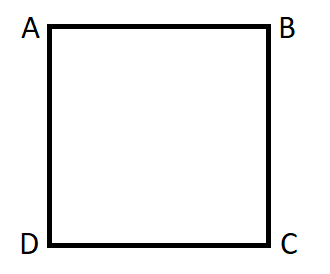
\includegraphics[scale=0.7]{DC_geometry}
\caption{Geometry of the driven cavity problem}\label{fg:DC_geometry}
\end{figure}  

Mathematically the problem to be solved is
\begin{equation}
\left \{
\begin{array}{rccl}
- \nabla \cdot (2 \mu \overline{\overline{\varepsilon}}) + \rho 
\vec{u} \cdot \nabla \vec{u} + \nabla p & = & 0 & \mbox{ in } \Omega \\
\nabla \cdot \vec{u} & = & 0 & \mbox{ in } \Omega \\
\end{array}
\right .
\end{equation}
%
with the boundary conditions
\begin{equation}
\left \{
\begin{array}{rccl}
u_x & = & 4 	 & \mbox{ on } \Gamma_{A-B} \\
u_x & = & 0 & \mbox{ on } \Gamma_{B-C} \cup \Gamma_{C-D} \cup \Gamma_{D-A} \\
u_y & = & 0 & \mbox{ on } \Gamma  
\end{array}
\right .
\end{equation}
where $\mu$ is the viscosity, $\overline{\overline{\varepsilon}}$ is 
the strain tensor,  $\rho$ is the density, $\vec{u}$ is the velocity and
$p$ is the pressure. It is assumed that the density and viscosity are 
constants. 

\subsection*{Solution procedure}

The first step is the generation of a uniform computational mesh with 128 elements in the x and the y cartesian axis. This is achieved by the following input file for ElmerGrid which is stored in the "DrivenCavity.grd" file:

\ttbegin
*** ElmerGrid input file for structured grid generation ***
Version = 210903
Coordinate System = Cartesian 2D
Subcell Divisions in 2D = 1 1
Subcell Limits 1 = 0 1
Subcell Limits 2 = 0 1
Material Structure in 2D
  1
End
Materials Interval = 1 1
Boundary Definitions
! type out int double of the boundaries
  1     -1   1   1
  2     -2   1   1
  3     -3   1   1
  4     -4   1   1
End
Element Degree = 1
Surface Elements = 16384
\ttend

Then, import the file in ElmerGUI by selecting

\ttbegin
File
  Open -> DrivenCavity.grd
\ttend

This will generate a mesh which is visualized in Figure \ref{fg:DC_mesh}.

\begin{figure}[H]
\centering
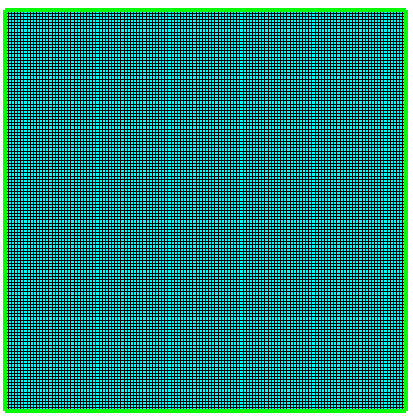
\includegraphics[scale=0.6]{DC_mesh}
\caption{The mesh for the driven cavity problem}\label{fg:DC_mesh}
\end{figure}

You can verify that the mesh consists of 16384 elements by inspecting the dialog box that appears when selecting

\ttbegin
Model
  Summary
\ttend

We can now define the model going through the Model menu from the top to bottom.  
In the equation section we choose the relevant equations and parameters related to their solution. 
We have only one set of equations which consists of the incompressible Navier-Stokes equation.

\ttbegin
Model
  Equation -> Add ..
\ttend  

We select the Navier-Stokes tab, click on the "Activate" box, apply the equation to "Body 1" and then click on the Ok button. The tab should look like Figure \ref{fg:DC_equation}. 

\begin{figure}[H]
\centering
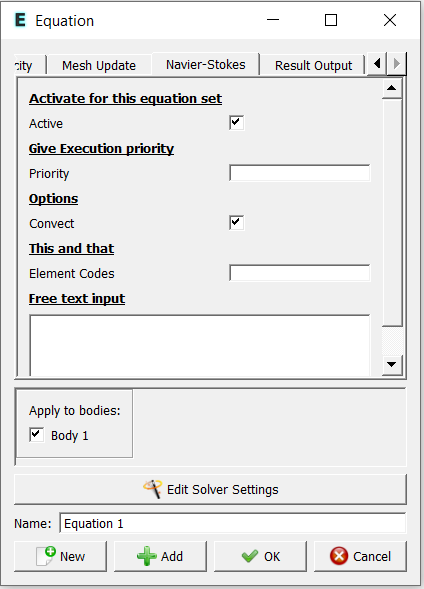
\includegraphics[scale=0.7]{DC_equation}
\caption{Equation}\label{fg:DC_equation}
\end{figure}

The Material section includes all material parameters. They are divided into generic parameters which are direct properties of the material without making any assumptions on the physical model, such as the density. Other properties assume a physical law, such as the viscosity. 
In the material section, we select 

\ttbegin
Model
  Material -> Add .. 
\ttend  

In the dialog box that appears, we first click on the General tab and we set the density equal to 1 and apply it to "Body 1" as shown in left panel of Figure \ref{fg:DC_material}.
Subsequently, we select the "Navier-Stokes" tab where we set the viscosity to 0.01, the "Compressibility model" to "Incompressible", apply it to "Body 1" and click ok as shown in the right panel of Figure \ref{fg:DC_material}.

\begin{figure}[H]
\centering
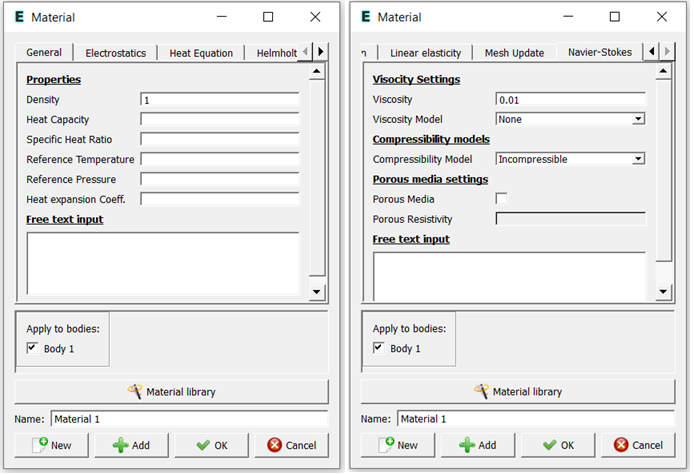
\includegraphics[width=0.8\textwidth]{DC_material}
\caption{Material properties}\label{fg:DC_material}
\end{figure}

For the linear system solvers we are happy to use the defaults. One may however, try out different preconditioners (ILU1,\ldots) or direct Umfpack solver, for example.

The appropriate boundary conditions can be set via  

\ttbegin
Model
  Boundary condition -> Add ..
\ttend

In the dialog box that appears, we select the "Navier-Stokes" tab. 
For the no slip condition on boundaries 1, 2 and 4 we click on the "No wall slip BC" option in the Navier-Stokes tab as shown in the left panel of Figure \ref{fg:DC_boundary}. 
For the case of lid velocity with 4 m/s in the x-direction and 0 m/s in the y-direction we specify the exact velocity values in the same tab when selecting "Boundary 3" as shown in the right panel of Figure \ref{fg:DC_boundary}.

\begin{figure}[H]
\centering
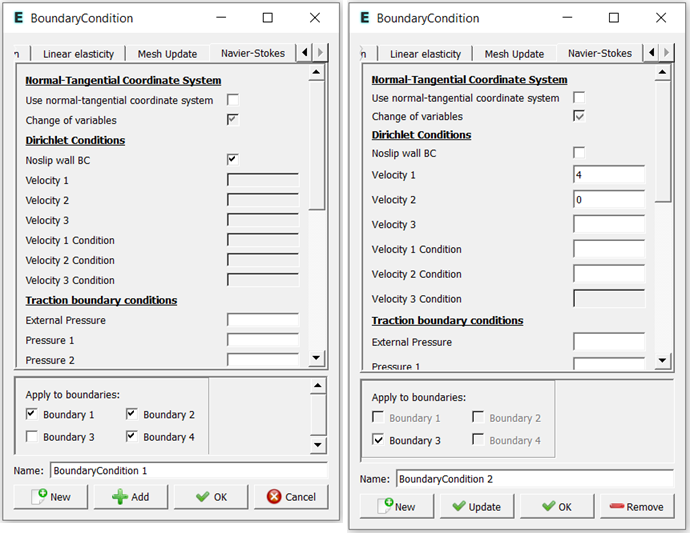
\includegraphics[width=0.8\textwidth]{DC_boundary}
\caption{Boundary conditions for the driven cavity}\label{fg:DC_boundary}
\end{figure}


For the execution, ElmerSolver needs the mesh files and the command file.  We can write and view the command file by selecting

\ttbegin
Sif 
  Generate
  Edit -> look how your command file came out  
\ttend

Before we can execute the solver we should save the files in a directory.  The ElmerGUI project includes all the files needed to restart the case.

\ttbegin
File 
  Save Project
\ttend

After we have successfully saved the files we may start the solver.

\ttbegin
Run
  Start solver
\ttend

A convergence view automatically pops up showing relative changes of each iteration. The problem should converge in less than ten iterations.
The variation of the residuals should be similar to the one in Figure \ref{fg:DC_convergence}. The required computational time should be a couple of minutes.

\begin{figure}[H]
\centering
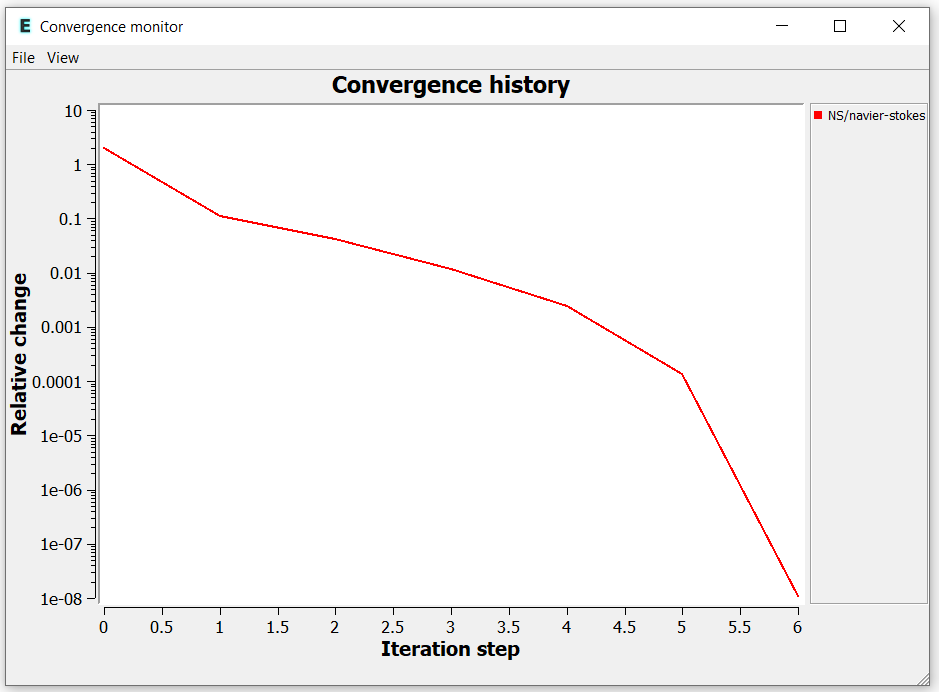
\includegraphics[scale=0.5]{DC_convergence}
\caption{Convergence of the solver.}\label{fg:DC_convergence}
\end{figure} 

When there are some results to view we may start the postprocessor:

\ttbegin
Run
  Start ParaView
\ttend

\subsection*{Results}


You may visualize the results with Paraview or ElmerVTK.
In Figure \ref{fg:DC_velocity_magnitude} the magnitude of the obtained velocity field is presented. The x- and y- cartesian components of the velocity vectors are shown in Figure \ref{fg:DC_velocity_x} and \ref{fg:DC_velocity_y}, respectively.

\begin{figure}[H]
\centering
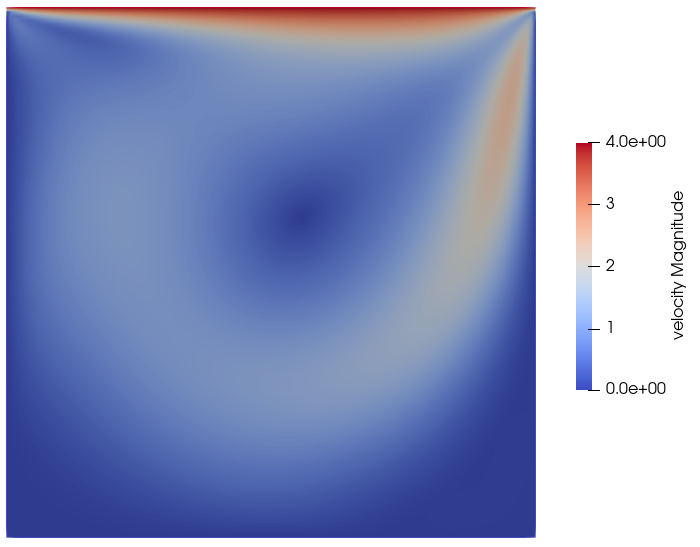
\includegraphics[scale=0.5]{DC_velocity_magnitude}
\caption{Distribution of velocity magnitude.}\label{fg:DC_velocity_magnitude}
\end{figure} 

\begin{figure}[H]
\centering
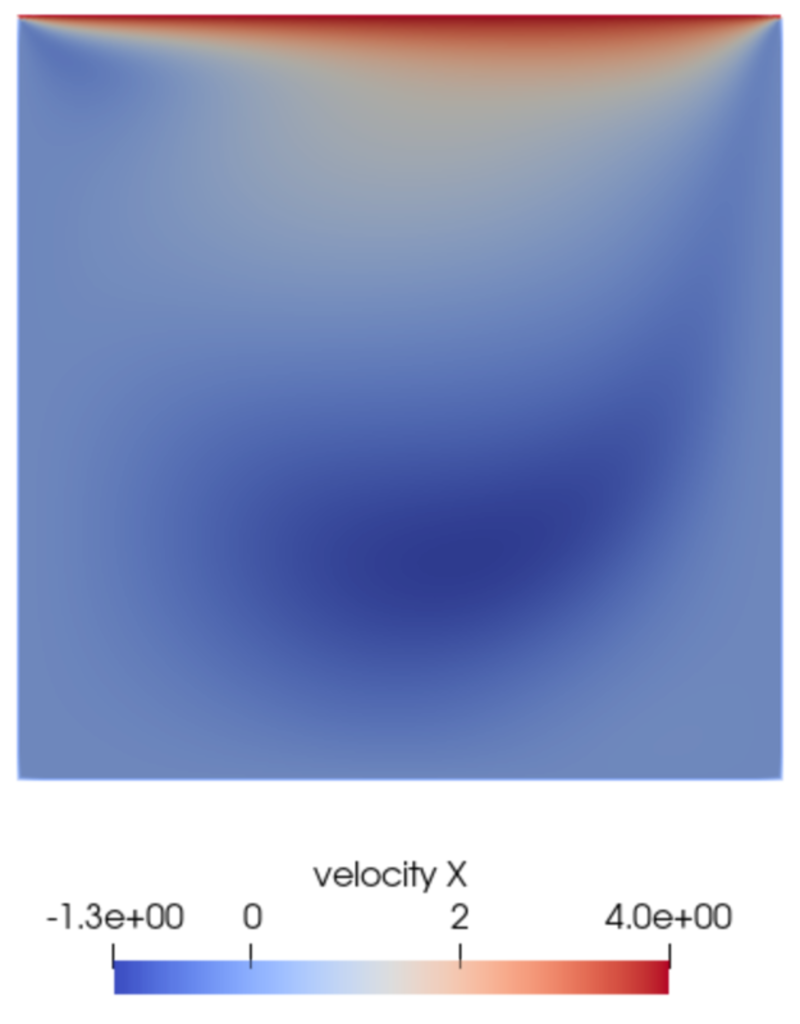
\includegraphics[scale=0.5]{DC_velocity_x}
\caption{Distribution of x-component of the velocity vector.}\label{fg:DC_velocity_x}
\end{figure} 

\begin{figure}[H]
\centering
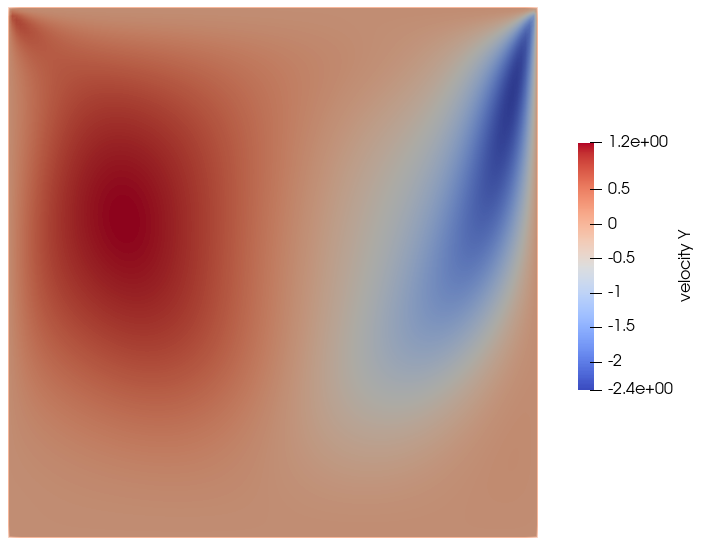
\includegraphics[scale=0.5]{DC_velocity_y}
\caption{Distribution of y-component of the velocity vector.}\label{fg:DC_velocity_y}
\end{figure} 

\subsection*{Extra task:}

You may try to solve the cases with parameters corresponding to Reynolds numbers of 100 and 3200.
This can be achieved by modifying the velocity of the upper boundary to 1 m/s and 32 m/s, respectively.
You can compare the obtained results with the data from the \href{https://www.grc.nasa.gov/www/wind/valid/cavity/cavity.html}{NASA repository}.

\hfill
